\section{Linear Feedback Shift Registers (LFSRs)}
The underlying idea of stream ciphers is the generation of a pseudorandom bit stream. An important tool for this are so called \textit{linear feedback shift registers (LFSRs)}. These kinds of shift registers are pseudorandom bit generators. This is by no means a new theory. Solomon Golomb wrote in 1967 in his book \textit{Shift Register Sequences} that the approach to generate pseudorandom sequences using LFSRs had been researched for two decades. \cite[p. 2]{Golomb.1967} Today, this idea has been developed further, resulting in many, partially theoretical applications that use shift registers. One reason for its popularity is its mathematical interpretability which is discussed in more detail in this chapter. 

\subsection{Generating Periodic Numbers}
A \textit{register} is a logical unit that has a certain number of \textit{memory cells}, each of which stores one bit of information. A set with $k$ of these cells forms a register. In the literature, no uniform term is used for these atomic elements of a register. Synonymous terms for the memory cells are, for example, \textit{memory elements} and \textit{stages} \cite[p. 81]{Stamp.2007}, \textit{delay elements} \cite[pp. 186-187]{Lidl.1986}, \textit{tubes} \cite[p. 27]{Golomb.1967} or, more broadly, \textit{bit sequence} \cite[p. 429]{Schneier.2006} or \textit{bit vector} \cite[p. 198]{Ertel.2020}. This paper uses the term memory cell as defined by Nigel P. Smart. \cite[p. 227]{Smart.2016} \\

The crucial factor of a \textit{feedback shift register} (FSR) is the connection of the memory cells via a feedback function $R$. After each clock signal, the register in its regular configuration shifts the contents of each cell to the next. In the process, one bit is shifted out at one end of the register. At the other end, a memory cell is freed. The sequence of these shifted out bits forms the sequence generated by the FSR. The new bit in the cleared memory cell at the other end is calculated by the function $R$ depending on the other bits. The shift direction differs in literature. In Smart and Schneier, for example, the shift is to the right \cite[p. 227]{Smart.2016}\cite[p. 429]{Schneier.2006} and in Lidl and Niederreiter to the left, which is adopted in this paper. The memory cell at the end where the content is shifted out has the least significant index $0$. The cell for which a new bit is calculated per clock signal has index $k-1$. \cite[pp. 186-187]{Lidl.1986}.
\begin{figure}[h]
	\centering
	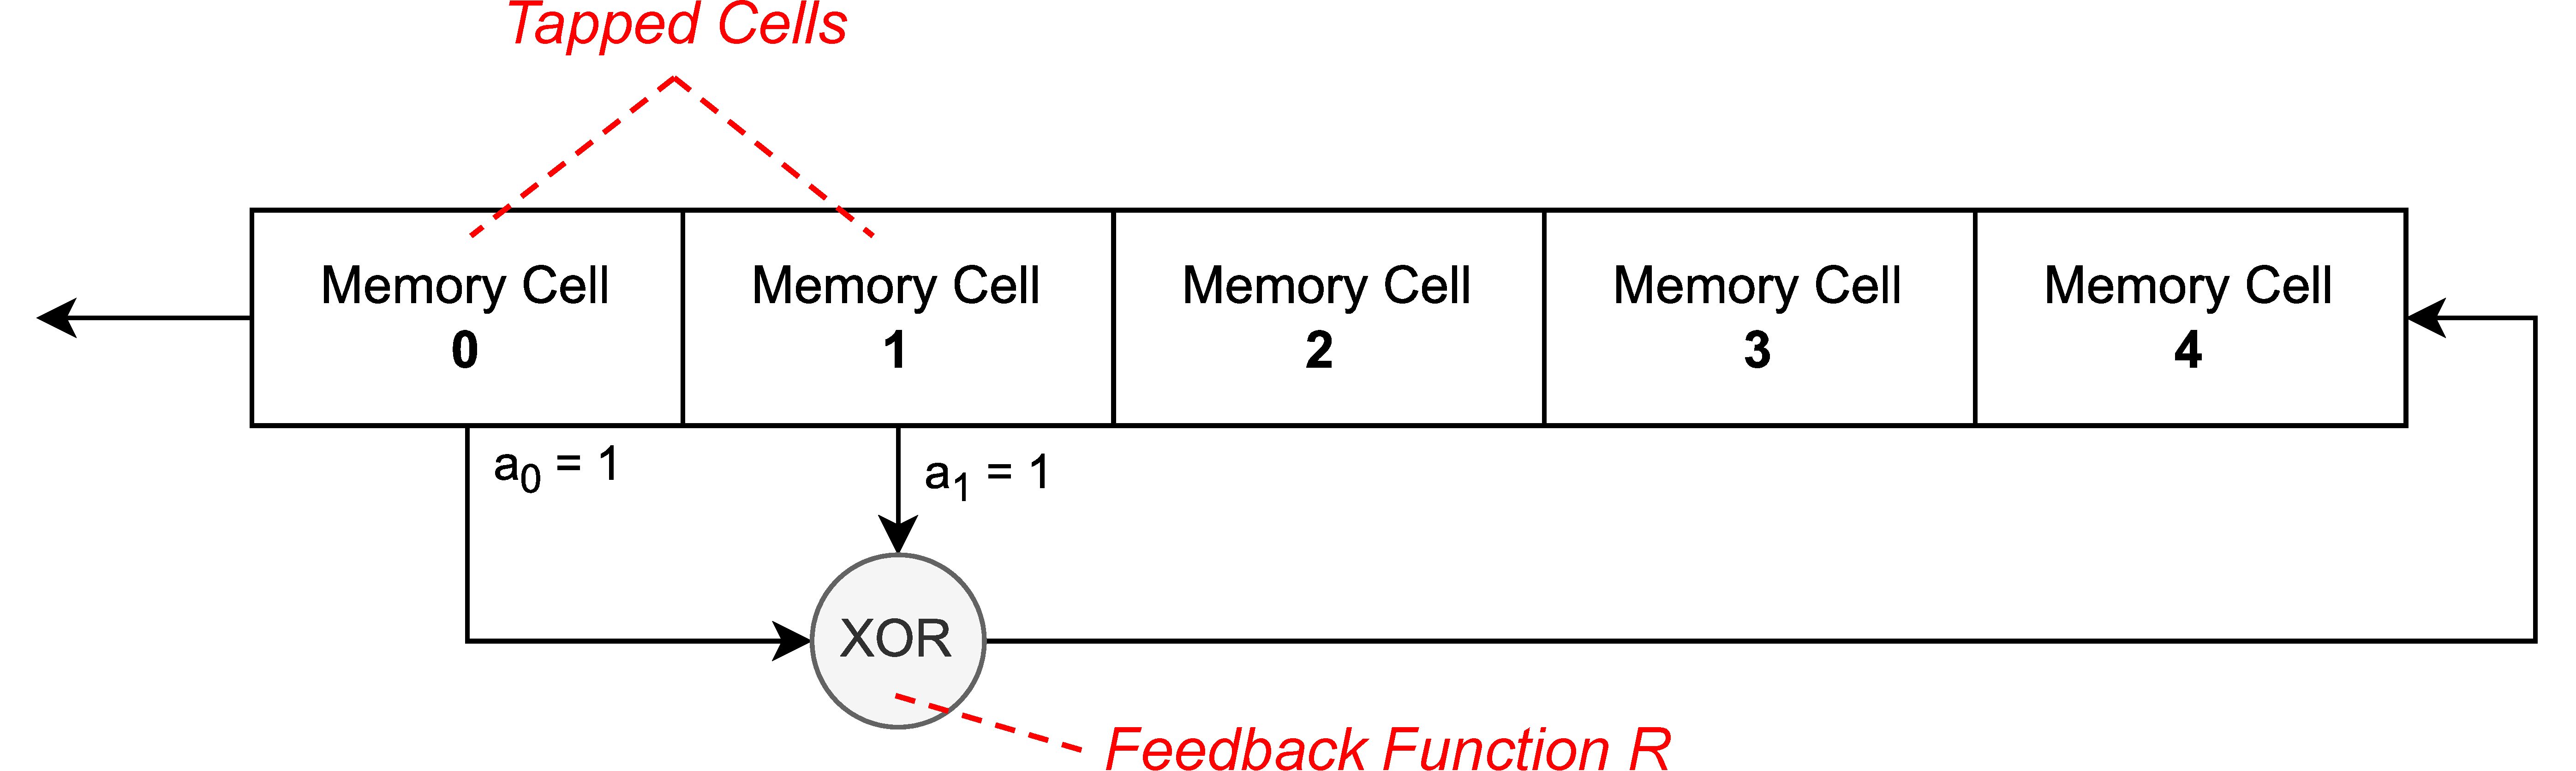
\includegraphics[width=1\linewidth]{carl/figures/figure_3_v4_svg-raw.pdf}
	\caption{Basic concept of an LFSR of length $k=5$. The linear XOR feedback function $R$ combines the values of the tapped memory cells $0$ and $1$. Based on \cite[p. 430]{Schneier.2006}}
	\label{fig:Figure_3}
\end{figure}

The characteristic aspect of a \textit{linear feedback shift register} (LFSR) is that the new bit $k-1$ is calculated by a linear feedback function. That means, certain memory cells calculate the new value of the freed cell with the binary addition XOR. \cite[p. 82]{Stamp.2007} These memory cells whose values are used for this calculation are called \textit{tapped} \cite[p. 227]{Smart.2016}. Analogous to LFSRs, nonlinear FSRs use feedback functions, with nonlinear elements, such as binary multiplication. This concept is introduced in chapter \ref{NLFSR}. Further details can be found in Lidl and Niederreiter, 1986, page 187. \\

In literature, LFSRs are described with different mathematical approaches. Common approaches use linear algebra, polynomial algebra and the theory of finite fields \cite[pp. 186ff.]{Lidl.1986}\cite[pp. 228ff.]{Smart.2016}. Less frequently, approaches with formal power series are chosen \cite[pp. 53ff.]{Beutelspacher.2005}\cite[pp. 201ff.]{Rueppel.1986}. In this paper, the first three approaches are investigated further. \\

\pagebreak

The sequence generated by an LFSR can be described as this relation:
\begin{equation*}
s_{n+k}=a_{k-1}s_{n+k-1}+a_{k-2}s_{n+k-2}+\ldots+a_0s_n+a \;\;\;\text{for}\; n = 0,1,\ldots
\end{equation*}

The variable $s_{n+k}$ represents the value of the newly calculated bit after $n$ clock signals, which changes state of the LFSR. The values $a_0,a_1,\ldots,a_{k-1}$ indicate the tapped memory cells. The constant $a$ will be explained later. If a memory cell $a_i$ is tapped, $a_i=1$, if not $a_i=0$. For an LFSR, $a$, $a_i$ and $s_i$ are elements of the finite field $\mathbb{F}_2$. This means they are elements of the Galois field of order $p=2$, where $p$ is a prime number. This corresponds to residue field $\mathbb{Z}/2\mathbb{Z}$. \cite[p. 48]{Lidl.1997} Initially, the LFSR of length $k$ is assigned the values $s_0,\ldots,s_{k-1}\in \mathbb{F}_2$. The generated sequence $s_0,s_1,\ldots,s_{k-1},s_k,\ldots,s_{k+n}$ is thus determined by the initial values. \cite[pp. 186-187]{Lidl.1986} \\

Figure \ref{fig:Figure_4} shows an LFSR of length $k=5$ with the initial state: $s_0=1, s_1=1, s_2=0, s_3=1$ and $s_4=1$. The memory cells $0$ and $1$ are tapped, resulting in $a_0=1$ and $a_1=1$ with the remaining $a_i=0$. After a clock signal, the binary addition $a_0s_0+a_1s_1=1\cdot1+1\cdot1=0$ generates the new bit $s_{k-1+1}=s_{4+1}=s_5$, which is inserted in the freed cell after the shift 

\begin{figure}[h]
	\centering
	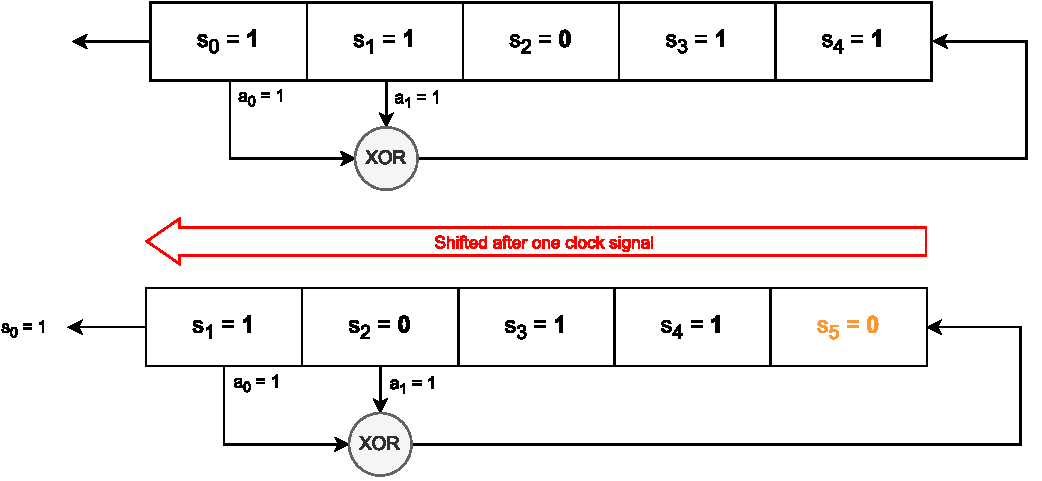
\includegraphics[width=0.9\textwidth]{carl/figures/figure_4_svg-raw.pdf}
	\caption{Workflow of an LFSR: After a clock signal, a new bit is calculated and the values of the memory cells are shifted to the left.}
	\label{fig:Figure_4}
\end{figure}

The sequence of shifted-out bits generated by an LFSR of length $k$ is called a \textit{$k$-th-order linear recurring sequence}. A distinction is made between \textit{homogenous} $k$-th-order linear recurring sequences when $a=0$ and \textit{inhomogeneous} $k$-th-order linear recurring sequence when $a\neq0$. The last case corresponds to the addition of a constant value in $\mathbb{F}_2$ to the equation above. \cite[p. 186]{Lidl.1986} Since LFSRs are usually constructed to produce homogenous $k$-th-order linear recurring sequences, the case $a\neq0$ is not considered further here. \\

As the name suggests, it is characteristic of $k$-th-order linear recurring sequences that they will repeat. A sequence is said to be \textit{periodic} if it will repeat after $r\in\mathbb{N}$ generated bits, such that $s_{n+r}=s_n$ for all $n\in\mathbb{N}_0$, where $r$ denotes the period of the sequence. This periodic behavior can possibly occur after $n_0\in\mathbb{N}_0$ non-periodic bits, such that: $s_{n+r}=s_n$ for all $n\ge{n_{0}}$. In this case the sequence is referred to as \textit{ultimately periodic} and $n_0$ as \textit{preperiod}. Any $k$-th-order linear recurring sequence with elements of $\mathbb{F}_2$ generated by an LFSR of length $k$ is ultimately periodic. The period $r$ takes at most the value $r\le2^{k}-1$. This can be explained since a register of length $k$ can only hold $2^{k}-1$ non-zero states. To avoid the trivial zero period, an LFSR of length $k$ must not be initialized with the zero sequence $s_0=s_1=\ldots=s_{k-1}=0$. \cite[p. 189]{Lidl.1986} \\

Figure \ref{fig:Figure_5} shows how the LFSR of length $k=5$ from the previous example generates a sequence of period $r=3$. The register returns to the initial state after $3$ clock signals. The preperiod is $n_0=0$.

\begin{figure}[h]
	\centering
	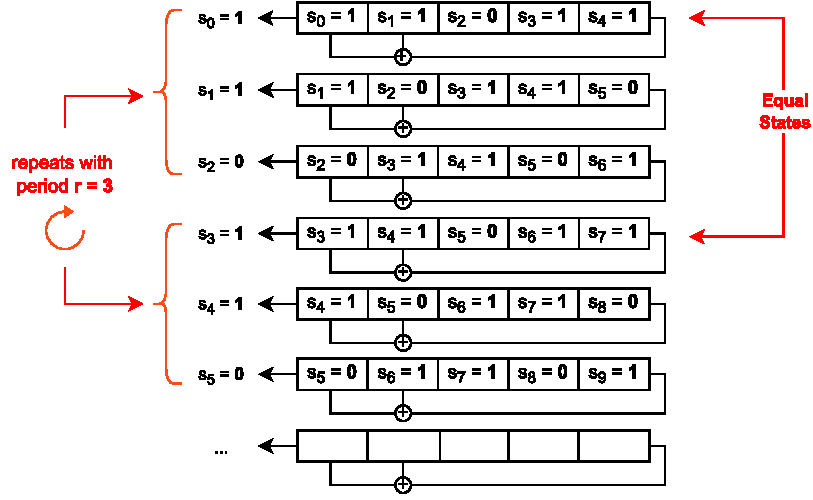
\includegraphics[width=0.75\textwidth]{carl/figures/figure_5_svg-raw.pdf}
	\caption{Periodic behavior of an LFSR. Once the state of an LFSR occurs a second time, the generated sequence will repeat.}
	\label{fig:Figure_5}
\end{figure}

Depending on the chosen values for $s_0,\ldots,s_{k-1}\in \mathbb{F}_2$ a different sequence with a possibly different period can be obtained. This can be illustrated by the following example: For each period, a state diagram is plotted. State $i$ in the diagram corresponds to an inner state of the LFSR in decimal notation. This state is formed by the contents of the memory cells $0$ to $k-1$ at a point in time. A state transition is created by applying the feedback function $R$. This representation is adapted from Nigel P. Smart in \cite[pp. 230]{Smart.2016}. Figure \ref{fig:Figure_6} shows all $32$ states of the LFSR of length $k=5$ from the previous two examples. 

\begin{figure}[h]
	\centering
	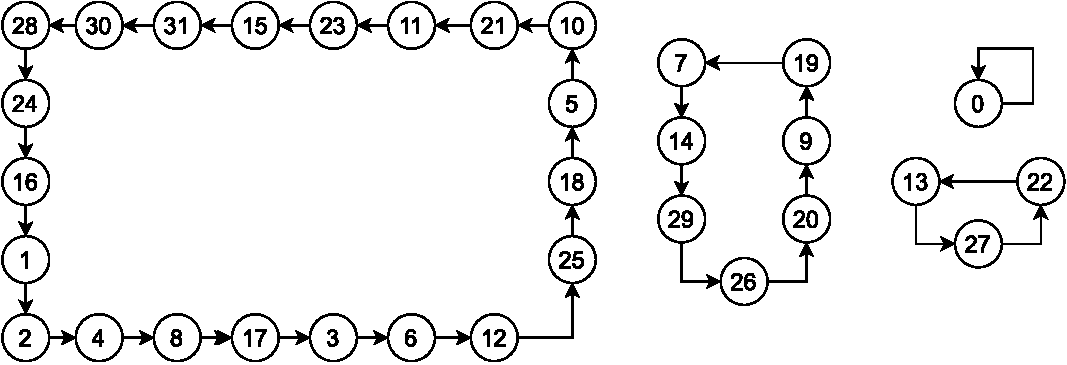
\includegraphics[width=0.87\textwidth]{carl/figures/figure_6_new_svg-raw.pdf}
	\caption{Representation of different periods of an LFSR as state machine diagrams. Based on \cite[pp. 230-232]{Smart.2016}}
	\label{fig:Figure_6}
\end{figure} 

\pagebreak

\subsection{m-sequences with Primitive Polynomials}
Consequently, the ultimate goal is to generate a pseudorandom number with the largest possible period. One option of trial and error is to select other tapped memory cells and check if the period has improved. Additionally, the choice of initialization values is limited, since different values for the same register may produce sequences with different periods. Such an effort is unfavorable for a symmetric encryption system. The most favorable situation would be to always generate a sequence with the largest possible period for an LFSR, regardless of the initialization vector chosen.\\

To achieve this situation, a second way must be presented to describe homogeneous $k$-th-order linear recurring sequences: An LFSR of length $k$ can be represented as the following regular $k\times{k}$ matrix $A$ over $\mathbb{F}_2$: the matrix elements $e$ in the diagonal below the main diagonal are assigned $1$: $e_{2,1},e_{3,2},\ldots,e_{k,k-1}=1$. The values of the tapped memory cells $a_i$ as defined above, are written in the $k$-th column in ascending order by index. \cite[p. 191]{Lidl.1986} For consistency, the notation of the matrix was adopted from Lidl and Niederreiter. Nigel P. Smart transposes the matrix \cite[p. 218]{Smart.2016}. As a result, the matrix $A\in \mathbb{F}_2^{k\times{k}}$ has this form:

\begin{equation*}
	\begin{pmatrix}
		0&0&0&\ldots&0&a_0\\
		1&0&0&\ldots&0&a_1\\
		0&1&0&\ldots&0&a_2\\
		\vdots&\vdots&\vdots&\ &\vdots&\vdots\\
		0&0&0&\ldots&1&a_{k-1}\\
	\end{pmatrix}
	\;\;\;\text{if }k=1,A\;\text{is the}\; 1 \times 1\;\text{matrix}\; (a_0)
\end{equation*}

The crucial point is the examination of the characteristic polynomial $f(x)$ of the matrix: 

\begin{equation*}
	f(x)=det(xI-A)=x^k-a_{k-1}x^{k-1}-a_{k-2}x^{k-2}-\ldots-a_0\in\mathbb{F}_2[x]
\end{equation*}

In the case of an LFSR, this polynomial is an element of the polynomial ring
$\mathbb{F}_2[x]$ over the finite field $\mathbb{F}_2$. Therefore, the coefficients of the polynomial – meaning the tapped memory cells – are elements of the finite field $\mathbb{F}_2$ \cite[pp. 18-19]{Lidl.1997}. Therefore, the signs of the coefficients before the indeterminant $x$ can be reversed:

\begin{equation*}
	f(x)=x^k+a_{k-1}x^{k-1}+a_{k-2}x^{k-2}+\ldots+a_0\in \mathbb{F}_2[x]
\end{equation*}

Only with the use of this characteristic polynomial it is possible to construct an LFSR which generates so-called \textit{maximal period sequences} with elements of $\mathbb{F}_2$. This refers to a sequence with the largest possible period and without preperiod, generated by an LFSR for any initial values except $0$. These sequences are also denoted as \textit{m-sequences}. Such sequences are generated by an LFSR of length $k$ if the characteristic polynomial of the matrix $A$ is a so-called \textit{primitive polynomial} in $\mathbb{F}_2[x]$. The period for all initial values except the zero initialization is $2^{k}-1$. \cite[p. 201]{Lidl.1986} \\

In the literature it is difficult to find a coherent and uniform explanation to primitive polynomials. For this paper the approach of Lidl and Niederreiter via finite fields was chosen.\\

Defining a primitive polynomial starts with the polynomial $f$ in $\mathbb{F}_2[x]$ of degree $m\ge1$. For an element $\alpha$ in $\mathbb{F}_{2^m}$ it must hold that $f(\alpha)=0$ is satisfied, whereby $\alpha$ is called the \textit{root} of $f$. The finite field $\mathbb{F}_{2^m}$ consists of the elements of $\mathbb{F}_2[x]$ modulus the polynomial $f$, resulting in $\mathbb{F}_{2^m}=\mathbb{F}_2[x]/f(x)$. \cite[p. 11]{Smart.2016} At the same time, $f$ must be the so-called \textit{minimal polynomial} of $\alpha$: Besides the property $f(\alpha)=0$, it must not be possible to factor it into further polynomials in $\mathbb{F}_2[x]$ of degree greater $0$. This property is comparable to that of a prime number. Moreover, if there is a polynomial $g$ in $\mathbb{F}_2[x]$ for which also holds $g(\alpha)=0$, then $g$ must divide the minimal polynomial $f$. The crucial characteristic of a minimal polynomial $f$ is that it is the polynomial of minimal degree with $f(\alpha)=0$, where the leading coefficient must be $1$. For this polynomial $f$ to be finally a primitive polynomial, it must hold that $\alpha$ generates the multiplicative group $\mathbb{F}_{2^m}^\times$. This group is equal to $\mathbb{F}_{2^m}$ without the $0$. Thus $\langle\alpha\rangle=\mathbb{F}_{2^m}^\times$ must hold. \cite[pp. 23, 31, 89]{Lidl.1997} \\

Just as it is difficult to test whether a number is prime, it is complex to find out whether a polynomial is primitive. \cite[p. 431]{Schneier.2006} Therefore, in the following example, we will only show that a given primitive polynomial satisfies the properties above: \\

Given is the primitive polynomial $f(x)=x^4+x^1+1$ in $\mathbb{F}_2[x]$ of degree $m=4$. For $\alpha \in \mathbb{F}_{2^4}$ holds $f(\alpha)=0$. This is how the finite field $\mathbb{F}_{2^4}=\mathbb{F}_2[x]/(x^4+x^1+1)$ is composed:
\vspace{-0.5 cm}
\begin{center}
	\begin{tabular}{l l l l l l l l}
		   	$0$	& 	$1$ \\
			$\alpha$	&	$\alpha+1$ \\
			$\alpha^2$	&	$\alpha^2+1$	&	$\alpha^2+\alpha$	&	$\alpha^2+\alpha+1$ \\ 
			$\alpha^3$	&	$\alpha^3+1$	&	$\alpha^3+\alpha$	&	$\alpha^3+\alpha+1$	&	$\alpha^3+\alpha^2$ 	&	$\alpha^3+\alpha^2+1$	&
			$\alpha^3+\alpha^2+\alpha$	& $\alpha^3+\alpha^2+\alpha+1$
	\end{tabular}
\end{center}
It can be assumed that the polynomial $f$ is a minimal polynomial. Now it will be shown that $\langle\alpha\rangle=\mathbb{F}_{2^m}^\times$, meaning that $\alpha$ generates the multiplicative group $\mathbb{F}_{2^m}^\times$.
\begin{center}
	\begin{tabular}{c c}
		$\begin{aligned}[t] % placement: default is "center", options are "top" and "bottom"
			\alpha^1 &= \alpha\\
			\alpha^2 &= \alpha^2 \\
			\alpha^3 &= \alpha^3 \\
			\alpha^4 &= \alpha + 1 \\
			\alpha^5 &= \alpha(\alpha^4)=\alpha(\alpha+1) \\
					 &= \alpha^2 + \alpha \\
			\alpha^6 &= \alpha^2\alpha^4 = \alpha^2(\alpha+1) \\
					 &= \alpha^3 + \alpha^2 \\
			\alpha^7 &= \alpha^3\alpha^4 = \alpha^3(\alpha+1) = \alpha^4\alpha^3 \\
					 &= \alpha^3+\alpha+1 \\
			\alpha^8 &= \alpha^4\alpha^4 = (\alpha + 1)(\alpha+1) \;\;\;\;\;\;\;\;\;\;\;\;\;\;\;\;\;\;\; \\
					 &= \alpha^2 + 2\alpha + 1 \\
					 &= \alpha^2 + 1 \\
			\alpha^9 &= \alpha^5\alpha^4 = (\alpha^2+\alpha)(\alpha+1) \\
					 &= \alpha^3 + \alpha^2 + \alpha^2 + \alpha \\
					 &= \alpha^3 + \alpha \\
			\alpha^{10}&= \alpha^5\alpha^5 = (\alpha^2+\alpha)(\alpha^2+\alpha) \\
					 &= \alpha^4 + 2\alpha + \alpha^2 \\
					 &= \alpha^2 + \alpha + 1 \\
		\end{aligned}$
		& 
		$\begin{aligned}[t] % placement: default is "center", options are "top" and "bottom"
			\alpha^{11} &= \alpha^5\alpha^6 = (\alpha^2+\alpha) (\alpha^2 + \alpha) \\
						&= \alpha^5+\alpha^4+\alpha^4+\alpha^3 \\
						&= \alpha^3+\alpha^2+\alpha \\
			\alpha^{12} &= \alpha^6\alpha^6 = (\alpha^3+\alpha^2)(\alpha^3+\alpha^2) \\
						&= \alpha^6 + 2\alpha^5 + \alpha^4 \\
						&= \alpha^3+\alpha^2+\alpha+1 \\
			\alpha^{13} &= \alpha^6\alpha^7 = (\alpha^3+\alpha^2)(\alpha^3+\alpha+1) \\
						&= \alpha^6 + \alpha ^4 + \alpha^3 + \alpha^5 + \alpha^3 + \alpha^2 \\
						&= \alpha^3 + \alpha^2 + \alpha + 1 + \alpha^2 + \alpha + \alpha^2 \\
						&= \alpha^3 + \alpha^2 + 1 \\
			\alpha^{14} &= \alpha^7\alpha^7 = (\alpha^3 + \alpha + 1)(\alpha^3 + \alpha + 1) \\
						&= \alpha^6 + \alpha^2 + 1 + 2\alpha^3\alpha + 2\alpha^3 + 2\alpha \\
						&= \alpha^3 + \alpha^2 + \alpha^2 + 1 \\
						&= \alpha^3 + 1 \\
			\alpha^{15} &= \alpha^8\alpha^7 = (\alpha^2 + 1)(\alpha^3 + \alpha + 1) \\
						&= \alpha^5 + \alpha^3 + \alpha^2 + \alpha^3 + \alpha + 1 \\
						&= \alpha^2 + \alpha + \alpha^2 + \alpha + 1\\
						&= 1
		\end{aligned}$
	\end{tabular}
\end{center}

\pagebreak

Consequently, $f(x)=x^4+x^1+1$ satisfies the properties of a primitive polynomial. The corresponding LFSR shown in figure \ref{fig:Figure_7} can be obtained with the help of the definition of the characteristic polynomial introduced previously: $f(x)=x^k+a_{k-1}x^{k-1}+a_{k-2}x^{k-2}+\ldots+a_0\in \mathbb{F}_2[x]$ \\

\begin{figure}[h]
	\centering
	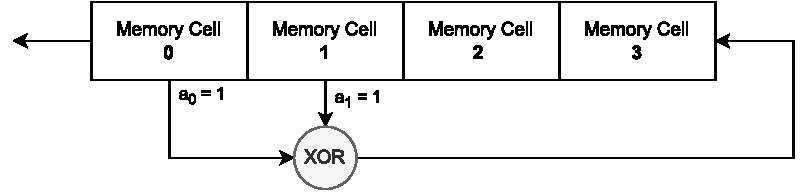
\includegraphics[width=0.9\textwidth]{carl/figures/figure_7_new_svg-raw.pdf}
	\caption{Structure of the LFSR which corresponds to the primitive polynomial $f(x)=x^4+x^1+1$,  based on \cite[p. 430]{Schneier.2006}}
	\label{fig:Figure_7}
\end{figure} 

The corresponding state machine diagram for this LFSR of length $k=4$ is shown in figure \ref{fig:Figure_8}. As can be seen, apart from the trivial zero period, only one period with maximum length $2^{k}-1=2^{4}-1=15$ exists. Thus, this LFSR, of which the characteristic polynomial is primitive, produces an m-sequence. 

\begin{figure}[h]
	\centering
	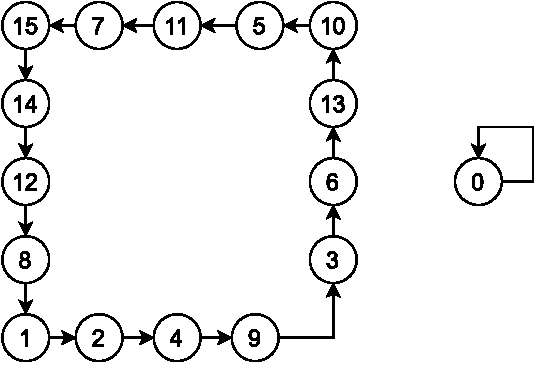
\includegraphics[width=0.51\textwidth]{carl/figures/figure_8_new_svg-raw.pdf}
	\caption{State machine diagram of the largest possible period of an LFSR whose characteristic polynomial is primitive. Based on  \cite[pp. 230-232]{Smart.2016}}
	\label{fig:Figure_8}
\end{figure}

Proof that such a primitive polynomial indeed generates an m-sequence is difficult to find in the literature. In many cases there are references to other authors or textbooks, without going into more detail or naming them. See, for example \cite[p. 229]{Smart.2016}. I wanted to have found a coherent explanation in the literature to the question: \textit{"Why do primitive polynomials in $\,\mathbb{F}_2[x]$ of degree $k$ generate sequences with maximum period $2^{k}-1$?"} For this paper, the example shown above should be sufficient. \\

In addition to having the longest possible period, m-sequences satisfy Solomon Golomb's randomness criteria mentioned initially \cite[p. 2847]{Gong.2018}. Thus, m-sequences are statistically secure pseudorandom numbers. However, the fact that a statistically secure pseudorandom number, such as the m-sequence, does not necessarily equal a cryptographically secure number will be discussed in the next chapter.

\pagebreak